\section{Sensores internos}
Los sensores internos se dividen en sensores de posición, de velocidad, de aceleración y de fuerza.

\subsection{Sensores de posición} Los sensores de posición miden la posición de cada articulación, es decir, el ángulo de articulación de un robot. A partir de dichos ángulos puede encontrarse la configuración del ejecutor final, y ubicar su posición y orientación por medio de la cinemática directa. A continuación se explican los diferentes sensores de posición.

\subsection*{Encoder incremental} El encoder es un dispositivo óptico digital que convierte el movimiento en una secuencia de pulsos digitales. Mediante el conteo de un solo bit o la decodificación de un conjunto de bits, los pulsos pueden convertirse en medidas relativas o absolutas. De este modo, los encóders son de tipo incremental o absoluto. Además, cada tipo puede ser lineal y rotatorio a su vez.

\begin{itemize}
	\item \textbf{Encoder lineal incremental:} Utiliza una escala con líneas opacas y espacios iguales en tamaño, ubicados en el rango de micrones. Una fuente de luz atraviesa la escala y es detectada por fotodiodos, generando pulsos cada vez que la luz es bloqueada. Estos pulsos actualizan un contador que mide la distancia recorrida.

	
	\item \textbf{Encoder rotativo incremental: } Similar al encoder lineal incremental, pero con retículas en un disco. Tiene dos conjuntos de líneas en diferentes círculos para detectar el sentido de rotación y mejorar la precisión. Además, cuenta con un círculo adicional con una sola marca para medir el número de revoluciones completadas.

	
\end{itemize}


\subsection*{Encoder absoluto}
\begin{itemize}
	\item \textbf{Encoder lineal absoluto: } Similar al incremental, pero proporciona un valor absoluto de la distancia en cualquier momento, evitando pérdida de pulsos a altas velocidades. Su salida es digital y utiliza una escala con secuencias de tiras opacas y transparentes que representan números binarios, permitiendo determinar la posición exacta.
	\item \textbf{Encoder rotativo absoluto: } Funciona como el encoder lineal absoluto, pero con un disco dividido en tiras circulares con segmentos de arco definidos. Proporciona una salida digital absoluta y se monta directamente en el eje del motor o con engranajes para mayor precisión. Para reducir errores, puede usar un código Gray, que evita confusiones en la salida binaria al cambiar solo un bit a la vez.
	
\end{itemize}


\begin{figure}[h]
	\centering
	\subfloat[Encoder]{%
		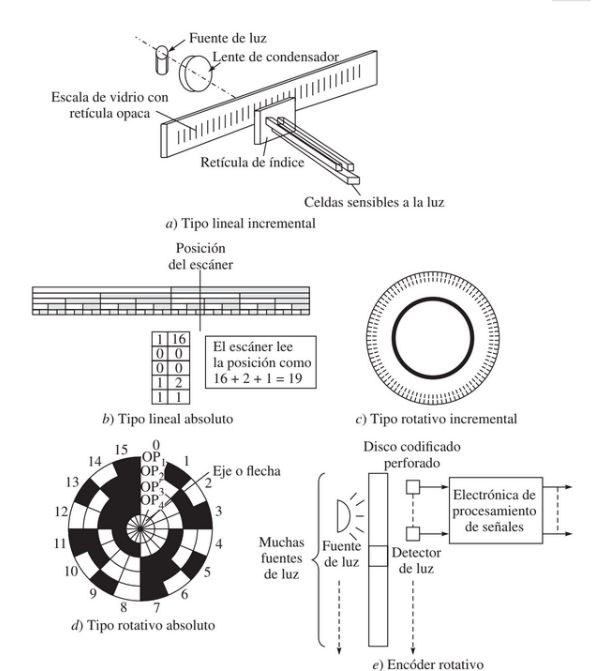
\includegraphics[width=0.8\textwidth]{Encoder.jpeg}%
		\label{fig:encoder}
	}
\end{figure}

\vspace{15cm}

\subsection*{Potenciometro}
\begin{itemize}
	\item \textbf{¿Qué hacen?} Es un dispositivo de resistencia variable que expresa desplazamientos lineales o angulares en términos de voltaje.
	\item \textbf{Principio de funcionamiento:} Consiste en una clavija deslizante que hace contacto con un elemento resistivo; conforme se mueve este punto de contacto, la resistencia entre el contacto deslizante y las conexiones de los extremos del dispositivo cambia en proporción al desplazamiento, x y  para potenciómetros lineales y angulares, respectivamente.
\end{itemize}	


\subsection*{Sensor LVDT}
\begin{itemize}
	\item \textbf{¿Qué hacen?} Los LVDT (transformadores diferenciales variables lineales) son sensores de posición lineal. Se utilizan para medir el desplazamiento lineal y la posición en distancias relativamente cortas. En la actualidad, existen LVDT en el mercado que pueden medir movimientos tan pequeños como varias millonésimas de cm (micro pulgadas) o incluso hasta aproximadamente 0,7 metros (~ 27 pulgadas) en el otro extremo. \cite{Dewesoft_LVDT} 
	
	Un LVDT consiste en un tubo que contiene un eje que se mueve libremente (también conocido como armadura). La base del tubo está montada en una posición fija y el extremo de la varilla se fija a un objeto cuya posición se moverá de forma lineal (hacia adelante y hacia atrás).
	
	\begin{figure}[h]
		\centering
		\subfloat[LVDT]{%
			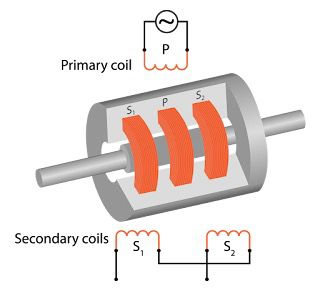
\includegraphics[width=0.4\textwidth]{lvdt.jpeg}%
			\label{fig:lvdt}
		}
	\end{figure}
	
	\item \textbf{Principio de funcionamiento:} Dentro de la carcasa del LVDT se encuentra la bobina primaria. A cada lado del conjunto de la bobina hay un par de bobinas secundarias. Excepto por sus posiciones físicas, los tres devanados primarios son idénticos. Sin embargo, están conectados en serie con la oposición, de modo que si se energizan por igual, sus salidas sumarán cero.
	
	Tenga en cuenta que estos elementos internos normalmente están construidos de tal manera que están protegidos contra la humedad y los campos magnéticos externos.
	
	\begin{figure}[h]
		\centering
		\subfloat[LVDT]{%
			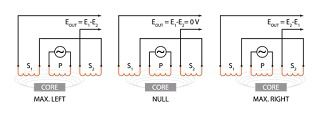
\includegraphics[width=0.6\textwidth]{lvdt2.jpeg}%
			\label{fig:lvdt2}
		}
	\end{figure}
	
	\vspace{15cm}
	
	\item \textbf{Tipos de LVDT o variedades mecánicas}
	
	En términos de su construcción de eje / armadura, existen varias variedades básicas disponibles en la actualidad:
	\begin{itemize}
		\item \text{LVDT de armadura libres (no guiados)} 
		\item \text{LVDT de armadura cautiva (guiada)} 
		\item \text{LVDT de armadura forzada o extendida por resorte} 
	\end{itemize}
	
	\item \textbf{Aplicaciones:} 
		\begin{itemize}
		\item \text{Herramientas de máquina} 
		\item \text{Bancos de prueba de tracción} 
		\item Prueba aeroespacial: tren de aterrizaje, actuadores, posicionamiento de la superficie de control, hidráulica
		\item \text{Ensayos de automoción y trenes: movimientos de los sistemas de suspensión}
		\item \text{Generación de energía: prueba de turbinas} 
		\item \text{Robótica: retroalimentación de posición} 
		\item \text{Fabricación: automatización, controles de procesos} 
		\item \text{Pulpa y papel - posicionamiento de los brazos tensores}
	\end{itemize}
\end{itemize}


\subsection*{Sensor Resólver}
\begin{itemize}
	\item \textbf{¿Qué hacen?} Un resolver es un sensor analógico de posición rotatoria, que a través de impulsos digitales puede regular la velocidad, la posición o el torque.
	
	El resolver consiste en una parte estacionaria llamada estator y una parte giratoria llamada rotor, que es montada al eje del motor. \cite{Servomotors_ResolverFeedback}
	
	\item \textbf{Principio de funcionamiento:} El bobinado primario del estator está conectado a una señal sinusoidal de alta frecuencia. Esta señal se transmite al bobinado del rotor, porque el bobinado primario del estator y el bobinado del rotor actúan juntos como un transformador. El campo magnético alternante pulsante del bobinado del rotor ahora induce una voltaje alterna en los bobinados de medición seno y coseno. Sus amplitudes, sin embargo, dependen de la posición angular del rotor.
	Si el bobinado del rotor y el bobinado de medición están paralelos el uno al otro, el campo del rotor magnético pasa completamente por la bobina de medición y, por lo tanto, el voltaje inducido es máximo.
	Sin embargo, si el bobinado del rotor y el bobinado de medición están en ángulos rectos el uno con el otro, no se producirá ningún voltaje.
	
	\item \textbf{Aplicaciones:} Los resolvers se utilizan en los servo motores para diferentes sectores industriales (Robótica, automoción, packaging, food and beverage, etc…) en los que se utilizan máquinas accionadas eléctricamente para procesos definidos. Ya que son sistemas de realimentación robustos y fiables que controlan el régimen de un servomotor de forma precisa.
	\item \textbf{Ventajas:}
	\begin{itemize}
		\item El propio resolver no contiene componentes electrónicos y por lo tanto puede soportar la temperatura caliente tan alta como 175 ° C y la temperatura baja tan bajo como -55 ° C.
		\item Un resolver es el dispositivo ideal retroalimentación confiable para su uso en condiciones ambientales adversas, ya que hay ninguna conexión eléctrica o mecánica entre el rotor y el estator.
		\item El rotor del resolver está montado directamente en el eje del motor, dando un sistema de medición robusto para señales de velocidad y posición.
		\item También puede alcanzar una velocidad de 90.000 rpm.
		\item Los resolvers no son susceptibles a la suciedad, aceite o ambientes calientes ya que los circuitos electrónicos están en otros dispositivos. Dispositivos como los encoders son más susceptibles a estas condiciones. Por eso, los resolvers han sido el dispositivo de realimentación escogido por muchos fabricantes.
	\end{itemize}
\end{itemize}
	\begin{figure}[h]
	\centering
	\subfloat[Resolver]{%
		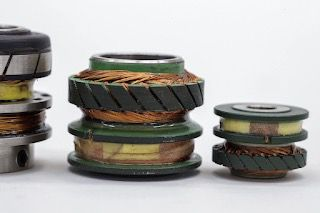
\includegraphics[width=0.4\textwidth]{resolver.jpeg}%
		\label{fig:resolver}
	}
\end{figure}



\subsection{Sensores de velocidad} Miden la velocidad a partir de cambios de posición en intervalos de tiempo constantes, calculando la razón de cambio respecto al tiempo de los valores de posición, o mediante diferentes principios.
\subsection*{Sensores de posición}
\begin{itemize}
	\item \textbf{¿Qué hacen?} Cualquier sensor de posición puede medir velocidad si se usa dentro de ciertos límites de tiempo. Por ejemplo, un encoder incremental calcula la velocidad dividiendo el número de pulsos entre el tiempo. Sin embargo, este método puede aumentar la carga computacional del controlador.
	
\end{itemize}
\subsection*{Tacómetro}
\begin{itemize}
	\item \textbf{¿Qué hacen?} Esencialmente, los tacómetros miden la velocidad de rotación de un elemento, utilizando el principio de que “el voltaje producido es proporcional al índice del acoplamiento inductivo”, por lo que el conductor (una bobina) se sujeta al elemento rotativo que gira en un campo magnético (estator), para que así, conforme se incremente la velocidad del eje, también aumente el voltaje producido en las terminales de las bobinas, pudiéndola medir directamente. 	\cite{BFMX_SensoresInternosRobot} 		
\end{itemize}

	\begin{figure}[h]
	\centering
	\subfloat[Tacometro]{%
		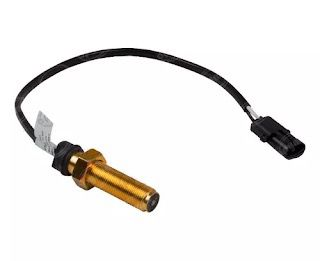
\includegraphics[width=0.4\textwidth]{tacometro.jpeg}%
		\label{fig:tcmtro}
	}
\end{figure}

\subsection*{Sensor de efecto Hall}
\begin{itemize}
	\item \textbf{¿Qué hacen?} Otro dispositivo de medición de velocidad es el sensor de efecto Hall, cuyo principio se describe a continuación. Si una pieza plana de material conductivo llamada chip Hall se sujeta a una diferencia de potencial en sus dos lados opuestos, entonces el voltaje que se genera a través de las caras perpendiculares es cero. Pero si un campo magnético se induce en ángulos rectos al conductor, el voltaje se genera en las otras dos caras perpendiculares. Entre más alto sea el valor de campo, más lo será el nivel de voltaje. Si se utiliza un imán anular, el voltaje producido será proporcional a la velocidad de rotación del imán. \cite{TE_Connectivity_Sensor}

\end{itemize}

	\begin{figure}[h]
	\centering
	\subfloat[Sensor de efecto Hall]{%
		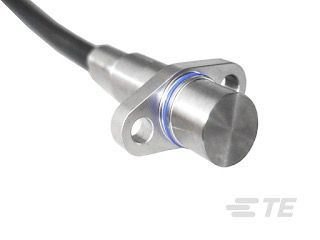
\includegraphics[width=0.4\textwidth]{sensorhall.jpeg}%
		\label{fig:sh}
	}
\end{figure}

\subsection{Sensores de aceleración} De manera parecida a las mediciones de velocidad que se dan a partir de la información de los sensores de posición, pueden encontrarse las aceleraciones como la razón de cambio respecto al tiempo de las velocidades obtenidas por los sensores de velocidad o calculado a partir de las informaciones de posición. Pero ésta no es una manera eficiente para calcular la aceleración, puesto que impondrá una carga de trabajo pesada sobre la computadora, lo que puede reducir la velocidad de operación del sistema. Otra forma de medir la aceleración es calculando la fuerza que resulta de multiplicar masa por aceleración. Las fuerzas se miden, por ejemplo, usando galgas extensométricas. 
\subsection*{Sensores de fuerza} 
\begin{itemize}
	\item \textbf{¿Qué hacen?} Una balanza de resorte es un ejemplo de un sensor de fuerza en donde se aplica una fuerza, por ejemplo, el peso, al platillo de balanza que causa un desplazamiento, es decir, el resorte se estira. El desplazamiento es entonces una medida de la fuerza. Existen otros tipos de sensores de fuerza, por ejemplo, con base en galgas, utilizando el sensor de efecto Hall, etcétera. 
\end{itemize}
\subsection{Sensores de fuerza}
\subsection*{Galgas extensiométricas}
\begin{itemize}
	\item \textbf{¿Qué hacen?} Las galgas extensiométricas son sensores cuya resistencia varía con la fuerza aplicada. Estos sensores convierten la fuerza, presión, tensión, peso, etc, en un cambio de la resistencia eléctrica el cual puede ser medido.
	\item \textbf{Principio de funcionamiento:} Cuando se aplica una fuerza externa a un objeto estacionario, se produce tensión y estrés sobre él. El estrés se define como las fuerzas internas de resistencia del objeto, y la tensión se define como el desplazamiento y la deformación que se producen.
	
	Las galgas extensiométricas son una de las herramientas más importantes en la técnica aplicada de medición eléctrica de magnitudes mecánicas. Como su nombre indica, se utiliza para la medición de tensiones. Se pueden utilizar para medir la expansión y la contracción.
	\item \textbf{Tipos:}
	\begin{itemize}
		\item \text{La Rejilla Karma o Serie K:} Rosetas T son para diseños de transductores de deformación axial, materiales Karma de precisión se desempeñan con buena linealidad en temperaturas de -75 a 200ºC (-100 a 392ºF), tienen un período de fatiga más largo.
		\item \text{Galgas extensiométricas de Precisión:} Propósito general, flexible, mecánicamente fuerte, radio de doblamiento pequeño, marcas de alineación claras, cables de cinta o terminación de soldadura, se puede utilizar con adhesivo frío o caliente; para mediciones de deformación dinámicas o estáticas altamente precisas.
		\item \text{Galgas extensiométricas Precableadas:} Salte el paso de soldadura en el punto de medición con los sensores precableados, sensores lineales de rejillas de 0,3 a 20 mm
		Rosetas T
		Rosetas planas de 0º, 45º, o 90º
		Sensores totalmente encapsulados para proteger el dispositivo de condiciones ambientales.
		\item \text{Galgas extensiométricas de calidad:} La serie SGT de galgas extensiométricas de calidad de transductor tiene rejillas paralelas dobles, para tensión de dobladura o de eje
		Aplicaciones de corte o torque
		Aplicaciones de transductor personalizadas de curva doble. \cite{Omega_GalgasExtensiometricas}
	\end{itemize}
\end{itemize}

\begin{figure}[h]
	\centering
	\subfloat[Galgas extensiometricas]{%
		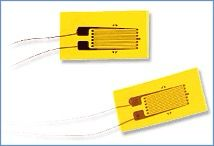
\includegraphics[width=0.4\textwidth]{galgas.jpeg}%
		\label{fig:galgas}
	}
\end{figure}



	\subsection*{Sensor piezoeléctrico}
\begin{itemize}
	\item \textbf{¿Qué hacen?} 
	Un material piezoeléctrico presenta un fenómeno conocido como efecto piezoeléctrico. Este efecto señala que cuando cristales elásticos asimétricos se deforman mediante una fuerza, se desarrollará un potencial eléctrico dentro de la red cristalina deformada. Este efecto es reversible. Esto quiere decir que si se aplica un voltaje entre las superficies del cristal, éste cambiará sus dimensiones físicas. La magnitud y polaridad de las cargas inducidas son proporcionales a la magnitud y dirección de la fuerza aplicada. Los materiales piezoeléctricos son cuarzo, turmalina, sal de Rochalle y otros. El rango de fuerzas que pueden medirse usando sensores piezoeléctricos es de 1 a 20 kN y con una proporción de $2*10^{5}.$ 
	Estos sensores pueden usarse para medir un cambio instantáneo en la fuerza (fuerzas dinámicas). \cite{IngMecafenix_SensorPiezoelectrico}
	
\end{itemize}

% Dos imágenes 
\begin{figure}[h]
	\centering
	\subfloat[]{%
		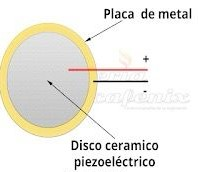
\includegraphics[width=0.4\textwidth]{piezoelectrico1.jpeg}%
		\label{fig:spe1}
	}
	\hfill
	\subfloat[]{%
		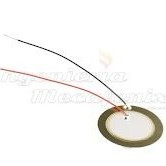
\includegraphics[width=0.4\textwidth]{piezoelectrico2.jpeg}%
		\label{fig:spe2}
	}
	\caption{Sensor piezoeléctrico}
	\label{fig:mascotas}
\end{figure}

\vspace{15cm}